\begin{figure}[ht]
\centering
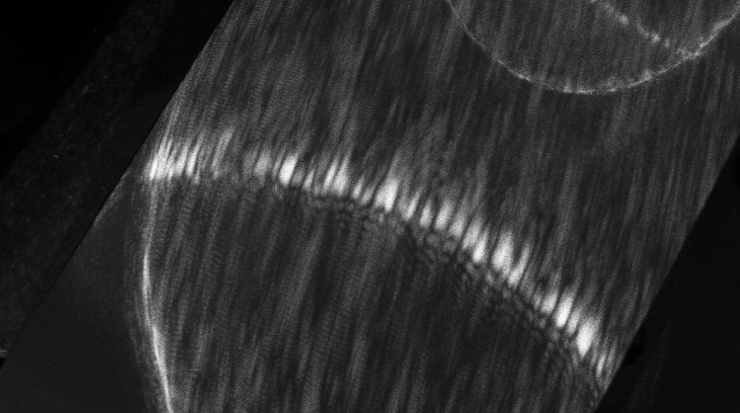
\includegraphics[keepaspectratio,width=15cm]{speckle/figures/Ag_LaSFN9_cone_lens11_cam-8899.jpg}
\caption{A portion of the cone speckle, distorted by a lens and projected on to a piece of paper.}
\label{fig:examplespeckle}
\end{figure}
\section{Introduction}
Under most circumstances, the intensity of light scattered in to the cone
is not spatially homogeneous, but exhibits distinctive intensity
fluctuations known as \textit{speckle}.  Such fluctuations arise due to the
interference of coherent waves with statistically random amplitudes and
phases.  Speckle in optics is closely related to the mesoscopic phenomena
of universal conductance fluctuations~\cite{lee1985universal}, and likewise
exhibits many of the same interesting physics such as coherent
backscattering~\cite{akkermans1986coherent} and the memory
effect~\cite{freund1988memory}.

As there is no prior work related to cone speckle, we begin with a basic
characterization of the speckle fields and compare them with theory.  In
particular we will look at the two most important characteristic properties
of speckle: size and contrast.  We omit any specific influence of the
changes in the underlying scattering microstructure, a topic reserved for
\Chapter{ch:scatteringmicro}.  
